\documentclass[onecolumn,10pt]{jhwhw}

\usepackage{epsfig} %% for loading postscript figures
\usepackage{amsmath}
\usepackage{graphicx}
\usepackage{grffile}
\usepackage{pdfpages}
\usepackage{algpseudocode}
\usepackage{wrapfig}
\usepackage{pgfplots}
\usepackage{amsfonts}
\usepackage{booktabs}
\usepackage{siunitx}
\usepackage{commath}

% Default fixed font does not support bold face
\DeclareFixedFont{\ttb}{T1}{txtt}{bx}{n}{12} % for bold
\DeclareFixedFont{\ttm}{T1}{txtt}{m}{n}{12}  % for normal

% Custom colors
\usepackage{color, colortbl}
\usepackage{listings}
\usepackage{framed}
\usepackage{caption}
\usepackage{bm}
\captionsetup[lstlisting]{font={small,tt}}

\definecolor{mygreen}{rgb}{0,0.6,0}
\definecolor{mygray}{rgb}{0.5,0.5,0.5}
\definecolor{mymauve}{rgb}{0.58,0,0.82}

\lstset{ %
  backgroundcolor=\color{white},   % choose the background color; you must add \usepackage{color} or \usepackage{xcolor}
  basicstyle=\ttfamily\footnotesize, % the size of the fonts that are used for the code
  breakatwhitespace=false,         % sets if automatic breaks should only happen at whitespace
  breaklines=true,                 % sets automatic line breaking
  captionpos=b,                    % sets the caption-position to bottom
  commentstyle=\color{mygreen},    % comment style
  deletekeywords={...},            % if you want to delete keywords from the given language
  escapeinside={\%*}{*)},          % if you want to add LaTeX within your code
  extendedchars=true,              % lets you use non-ASCII characters; for 8-bits encodings only, does not work with UTF-8
  frame=single,                    % adds a frame around the code
  keepspaces=true,                 % keeps spaces in text, useful for keeping indentation of code (possibly needs columns=flexible)
  columns=flexible,
  keywordstyle=\color{blue},       % keyword style
  language=R,                 % the language of the code
  % language=Python,                 % the language of the code
  morekeywords={*,...},            % if you want to add more keywords to the set
  numbers=left,                    % where to put the line-numbers; possible values are (none, left, right)
  numbersep=5pt,                   % how far the line-numbers are from the code
  numberstyle=\tiny\color{mygray}, % the style that is used for the line-numbers
  rulecolor=\color{black},         % if not set, the frame-color may be changed on line-breaks within not-black text (e.g. comments (green here))
  showspaces=false,                % show spaces everywhere adding particular underscores; it overrides 'showstringspaces'
  showstringspaces=false,          % underline spaces within strings only
  showtabs=false,                  % show tabs within strings adding particular underscores
  stepnumber=1,                    % the step between two line-numbers. If it's 1, each line will be numbered
  stringstyle=\color{mymauve},     % string literal style
  tabsize=4,                       % sets default tabsize to 2 spaces
}

\usepackage{amsmath,amssymb,mathtools,bm,etoolbox}

\providecommand\given{}
\DeclarePairedDelimiterXPP\Aver[1]{\mathbb{E}}{[}{]}{}{
\renewcommand\given{  \nonscript\:
  \delimsize\vert
  \nonscript\:
  \mathopen{}
  \allowbreak}
#1
}

\author{John Karasinski}
\title{Final}

\begin{document}
%\maketitle

\problem{}
(30 points) Imagine that you are interested in the relationship between mood and weather. You ask 4 people to fill out a questionnaire about their mood for 70 consecutive days and also record the maximum temperature of each day. The data for the weather and the mood from the 4 individuals are in the “tempmood.csv” data set.\\
\\
(a) Plot the data in a way/s that you find meaningful to examine the relationship between mood and weather. Interpret the graph/s.\\
\\
Two plots are generated here. The first is a scatter plot with the regression line between all subjects' mood and the temperature for all days ($n=4$). This plot is useful to show us the overall structure of the data---at this point I don't care that we measured data from multiple individuals, I just want to see if there is an immediate, obvious relationship between mood and temperature. We find $r=-.24$, suggesting that only~6\% of the variance in mood can be explained by temperature.

\begin{figure}[b!]
\begin{center}
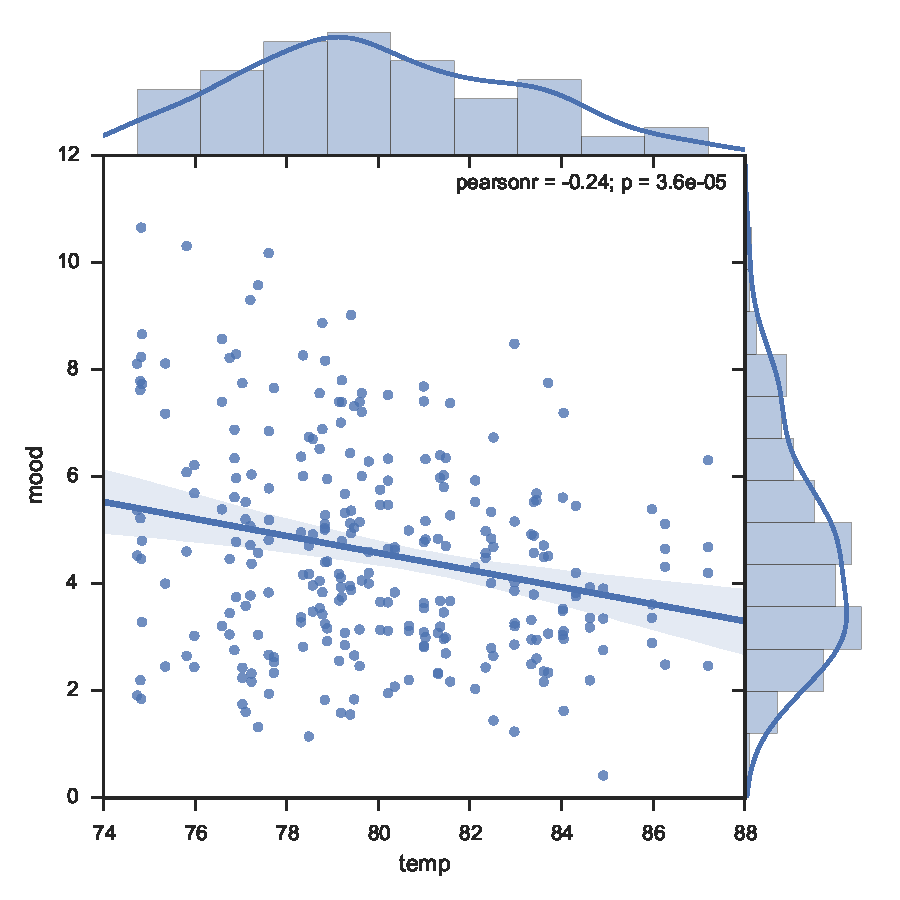
\includegraphics[height=0.5\textheight]{p1-mean.pdf}
\label{fig:on}
\end{center}
\caption{Scatter plot of each subject's mood vs temperature of for each day. Regression line shows a negative correlation between mood and temperature $(r=-0.24)$. }
\end{figure}
A second plot was made to investigate the correlations between individual subject's mood and the weather. Correlations between mood and temperature vary between subjects: $r_{T1} = .3, r_{T2} = 0, r_{T3} = -.3, r_{T4} = -.7$, and correlations between all pairs of subjects' moods are $\approx 0$. This plot tells us a lot more than the first. We now know that some subjects have a positive correlation between mood and weather, some have no correlation, and some have a negative (or very negative) correlation. Thanks to this plot, I see that there are very different responses among subjects, and that we will probably need to sample a larger number of subjects before we can draw meaningful conclusions about the population's relations between mood and weather.\\
\\
The code to make these plots:
\begin{figure}[t!]
\begin{center}
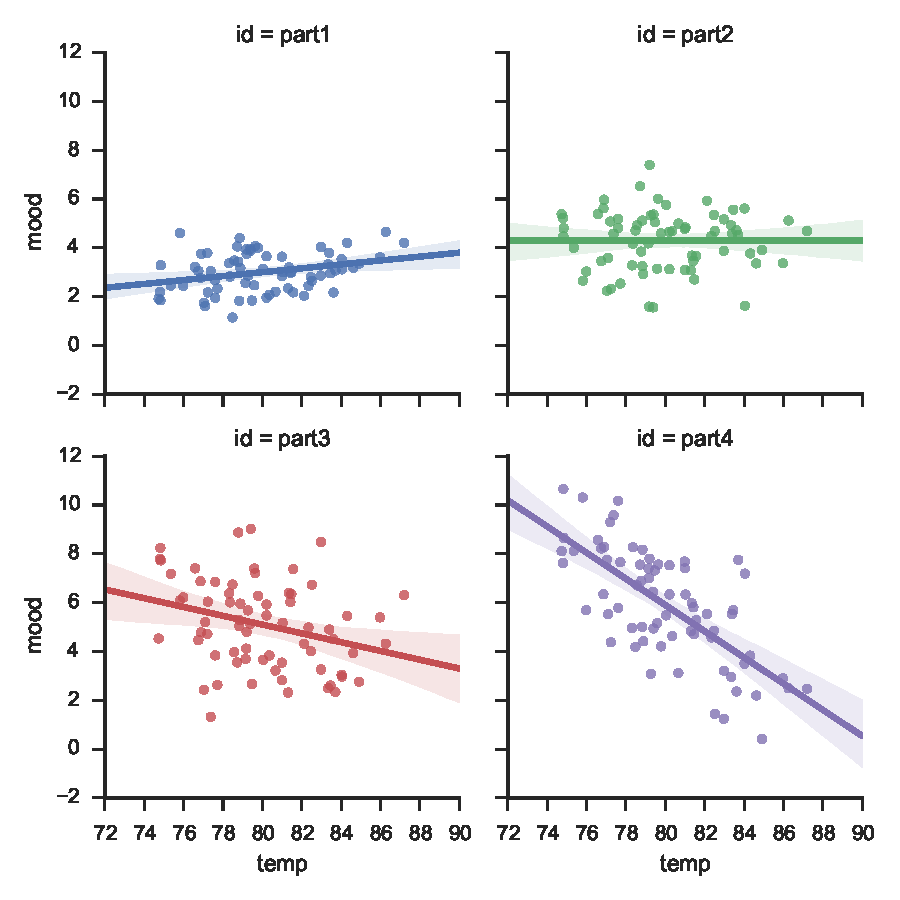
\includegraphics[height=0.5\textheight]{p1-persubj.pdf}
\label{fig:on}
\end{center}
\caption{Investigation of individual participant's relationships between mood and temperature.}
\end{figure}
\begin{lstlisting}[language=Python]
df = pd.read_csv('tempmood.csv')
df['day'] = df.index.tolist()
d = pd.melt(df, id_vars='temp', value_vars=['part1', 'part2', 'part3', 'part4'],
            value_name='mood', var_name='id')
sns.jointplot('temp', 'mood', data=d, xlim=(74, 88), ylim=(0, 12), space=0,
              kind='reg')
sns.lmplot(x='temp', y='mood', hue='id', col='id', col_wrap=2, data=d, size=3)
\end{lstlisting}

\clearpage
\noindent (b) Compute means and standard deviations for the data.
\begin{lstlisting}[language=Python]
stats = pd.DataFrame.from_dict({'mean':df.mean(), 'std':df.std()})
print(stats)
#             mean        std
# temp       80.00   3.000000
# part1       3.00   0.800000
# part2       4.30   1.200000
# part3       5.10   1.800000
# part4       5.90   2.300000
\end{lstlisting}

\noindent (c) Estimate the covariance between weather and mood as well as the sum of cross-products. What does each of these indices indicate about the relation between weather and mood?
\begin{lstlisting}[language=Python]
print(df.cov()['temp'])
# temp   9.000000e+00
# part1  7.200000e-01
# part2  2.569603e-15
# part3 -1.620000e+00
# part4 -4.830000e+00
print((df.cov() * (len(df) - 1))['temp'])
# temp   6.210000e+02
# part1  4.968000e+01
# part2  1.773026e-13
# part3 -1.117800e+02
# part4 -3.332700e+02
\end{lstlisting}
% The diagonal terms indicate the unbiased variance within each variable. (These variances are not very close to equal, suggesting that we may not be able to assume homogeneity of variance.) The off-diagonal elements show the unbiased covariances among the variables. We see that all of the indices relating two subjects are approximately zero. This suggests that the subjects' moods do not covary with each other. With the exception of the second subject, we see that subjects tend to have some non-zero covariance with temperature. This may indicate a significant correlation between some subject's mood and the temperature. The matrix of covariance is symmetric, as the covariance formula doesn't depend on the order of variables. To calculate the sum of cross-products, we simply multiply by $N-1$.\\
The first term indicates the unbiased variance within the temp variable. With the exception of the second subject, we see that subjects tend to have some non-zero covariance with temperature. This may indicate a significant correlation between some subject's mood and the temperature. To calculate the sum of cross-products, we simply multiply the covariance by $N-1$.\\
\\
(d) What is the correlation between weather and mood across all participants? What does the correlation indicate about the relationship between weather and mood?
\begin{lstlisting}[language=Python]
print(d.corr())
#           temp      mood
# temp  1.000000 -0.244438
# mood -0.244438  1.000000
\end{lstlisting}
There is a correlation of -0.24 between temperature and weather, indicating that a larger temperature corresponds to a lower mood. This also indicates that about ~6\% of the variance in mood is explained by weather. While there is no way for us to definitively say that a higher temperature \textit{causes} a lower mood, it seems unlikely that a lower mood causes a higher temperature. Despite this, higher temperatures may directly or indirectly cause lower mood, and the correlation does not imply causation.\\
\\
(e) Estimate the regression equation of the line that best represents the relationship between weather and mood for all individuals as a single group.
\begin{lstlisting}[language=Python]
import statsmodels.api as sm
def fit_line(x, y):
    """Return slope, intercept of best fit line."""
    X = sm.add_constant(x)
    model = sm.OLS(y, X)
    fit = model.fit()
    return fit.params[1], fit.params[0]

m, b = fit_line(d.temp, d.mood)
print("Slope: {:.2f} Intercept: {:.2f}".format(m, b))

# Slope: -0.16 Intercept: 17.31
\end{lstlisting}
The resulting regression line is then:
$$
Y_{\mbox{mood}} = 17.31 - 0.16 X_{\mbox{temp}}
$$
(f) Estimate the regression equation of the line that best represents the relationship between weather and mood for each individual.
\begin{lstlisting}[language=Python]
for i in range(1, 5):
   print("Subject: {:d}, Slope: {:+.2f} Intercept: {:+.2f}"
         .format(i, *fit_line(df.temp, df['part' + str(i)])))

# Subject: 1, Slope: +0.08 Intercept: -3.40
# Subject: 2, Slope: +0.00 Intercept: +4.30
# Subject: 3, Slope: -0.18 Intercept: +19.50
# Subject: 4, Slope: -0.54 Intercept: +48.83
\end{lstlisting}
For subjects 1-4, the resulting regression lines are:
\begin{align*}
Y_{1} = -3.40  +0.08 X_{\mbox{temp}}\\
Y_{2} = 4.30  +0.00 X_{\mbox{temp}}\\
Y_{3} = 19.50 -0.18 X_{\mbox{temp}}\\
Y_{4} = 48.83 -0.54 X_{\mbox{temp}}
\end{align*}
(g) Test whether the relation between temperature and mood is significantly different between persons using Fisher's z transformations and z-test.
\begin{lstlisting}[language=Python]
from scipy.stats import norm
t = df['temp']
m1 = df['part1']
m2 = df['part2']
m3 = df['part3']
m4 = df['part4']

res = []
for m_1 in [m1, m2, m3, m4]:
    mcor1  = pd.concat((t, m_1), axis=1).corr().temp[1]
    mcor1z = 0.5 * np.log((1+mcor1)/(1-mcor1))
    for m_2 in [m1, m2, m3, m4]:
        mcor2 = pd.concat((t, m_2), axis=1).corr().temp[1]
        mcor2z = 0.5 * np.log((1+mcor2)/(1-mcor2))
        zres = (mcor2z - mcor1z)/np.sqrt(2/(len(m_2)-3))
        p = 2*norm.sf(zres)
        res.append(p)
res = pd.DataFrame(np.array(res).reshape(4, 4))
labels = ['Subject' + str(i) for i in range(1, 5)]
res.columns, res.index = labels, labels

# Show just the lower triangular
print(res.mask(np.triu(np.ones(res.shape)).astype(np.bool)))

#               Subject1      Subject2  Subject3  Subject4
# Subject1           NaN           NaN       NaN       NaN
# Subject2  7.321723e-02           NaN       NaN       NaN
# Subject3  3.397377e-04  7.321723e-02       NaN       NaN
# Subject4  9.669450e-12  5.170788e-07  0.001245       NaN
\end{lstlisting}
(h) What can you say about differences in the relationship between weather and mood across individuals?\\
\\
Fisher's z-tests were used to determine if correlations between subject's moods and the weather were significantly different from each other. All subject's correlations were significantly different from each other at the $p=0.01$ level. This indicates that each pair of subjects' relation between temperature and mood was significantly different.\\
\\
(h) You submit the result of all these analyses for publication but the editor rejects the manuscript on the basis of: (i) a lack of power to examine your research questions, and (ii) the fact that there are only 4 individuals in your data and, thus---they claim---you cannot generalize to the population. Nevertheless, you are convinced---or just have a hunch---that there might be something valuable here and write back arguing that the data and analyses are worth disseminating. What would you say to support your argument?\\
\\
I would likely argue that, while these results may or may not be representative of the population, the results presented here are nonetheless interesting and statistically significant. I would concede that the correlation among all subjects, $r=-0.24$, is likely not representative of the population. Despite this, I would argue that there was significant power to significantly detect effects. While the sample size is not large, the magnitude of the effect size was enormous. As such, we still have enough power to detect significant effects at a relevant statistical significance criterion. Further, we have shown that individuals can have significant correlations between mood and weather, and that these can be significantly different from person to person.

\clearpage
\problem{}
(10 points) The following matrices RV and CV are a correlation and a covariance matrix, respectively, of variables $X_1$, $X_2$, $X_3$, $X_4$, and $X_5$. Using the information provided in the matrices, fill in the gray boxes with the appropriate values. Make a note of any anomalies you notice (if any).

\begin{table}[h!]
\begin{center}
\begin{tabular}{rr|rrrrr}
\toprule
  & & $X_1$ & $X_2$ & $X_3$ & $X_4$ & $X_5$ \\
\midrule
            & $X_1$ & \cellcolor{gray} 4     & -       & -     & -     & -   \\
            & $X_2$ & -0.5   & 0.25    & -     & -     & -   \\
Covariance  & $X_3$ & 1.8    & \cellcolor{gray}1.125       & \cellcolor{gray} 9    & -     & -   \\
            & $X_4$ & -1.08  & -0.135  & -2.43 & 7.29  & -   \\
            & $X_5$ & 17.28  & \cellcolor{gray} 1.35      &  6.48 & 4.374 & \cellcolor{gray} 29.16   \\
\midrule
            & $X_1$ & 1.0      & -       & -     & -     & -   \\
            & $X_2$ & -0.5   & 1.0       & -     & -     & -   \\
Correlation & $X_3$ & \cellcolor{gray} 0.3     & 0.25    & 1.0     & -     & -   \\
            & $X_4$ & \cellcolor{gray} -0.2      & \cellcolor{gray}-0.1       & -0.3  & 1.0     & -   \\
            & $X_5$ & \cellcolor{red} 1.6     & 0.5     & \cellcolor{gray}0.4     & 0.3   & 1.0   \\
\bottomrule
\end{tabular}
\end{center}
\end{table}
There is one anomaly, the correlation $r_{15} = 1.6 > 1$ is impossible. This stems from $c_{15}$ being artificially too large.
\begin{equation*}
\begin{aligned}[c]
s_{2}^2 &=0.25 \implies s_2 = 0.5 \\
s_{4}^2 &=7.29 \implies s_4 = 2.7 \\
& \Downarrow \\
r_{11} &= \frac{c_{11}}{s_1 s_1} \implies c_{11} = r_{11} s_{1} s_{1}\\
r_{13} &= \frac{c_{13}}{s_1 s_3} \\
r_{14} &= \frac{c_{14}}{s_1 s_4} \\
r_{15} &= \frac{c_{15}}{s_1 s_5} \\
r_{23} &= \frac{c_{23}}{s_2 s_3} \implies c_{23} = r_{23} s_{2} s_{3}\\
r_{24} &= \frac{c_{24}}{s_2 s_4} = \frac{-0.135}{(0.5)(2.7)} = -0.1\\
r_{25} &= \frac{c_{25}}{s_2 s_5} \implies c_{25} = r_{25} s_{2} s_{5}\\
r_{33} &= \frac{c_{33}}{s_3 s_3} \implies c_{33} = r_{33} s_{3} s_{3}\\
r_{35} &= \frac{c_{35}}{s_3 s_5} \\
r_{55} &= \frac{c_{55}}{s_5 s_5} \implies c_{55} = r_{55} s_{5} s_{5}
\end{aligned}
\qquad\implies\qquad
\begin{aligned}[c]
r_{12} &= \frac{c_{12}}{s_1 s_2} \implies s_1 = \frac{c_{12}}{r_{12} s_2} = \frac{-0.5}{(-0.5)(0.5)} = 2\\
r_{34} &= \frac{c_{34}}{s_3 s_4} \implies s_3 = \frac{c_{34}}{r_{34} s_4} = \frac{-2.43}{(-0.3)(2.7)} = 3\\
r_{45} &= \frac{c_{45}}{s_4 s_5} \implies s_5 = \frac{c_{45}}{r_{45} s_4} = \frac{4.374}{(0.3)(2.7)} = 5.4\\
& \Downarrow \\
c_{11} &= s_{1}^2 = 4\\
r_{13} &= \frac{1.8}{(2) (3)} = 0.3 \\
r_{14} &= \frac{-1.08}{(2) (2.7)} = -0.2 \\
r_{15} &= \frac{17.28}{(2) (5.4)} = 1.6\\
c_{23} &= (0.25) (0.5) (9) = 1.125\\
c_{25} &= (0.5) (0.5) (5.4) = 1.35\\
c_{33} &= s_{3}^2 = 9\\
r_{35} &= \frac{6.48}{(3) (5.4)} =0.4\\
c_{55} &= s_{5}^2 = 29.16
\end{aligned}
\end{equation*}

\clearpage
\problem{}
(20 points) Researchers were interested in the role of extracurricular activities (sports: 0 = other extracurricular activities and 1 = participation in sports) and biological sex (female: 0 = male, 1 = female) on standard normal adolescent perceptions of social acceptance (PSA). The data can be found in the “socialacceptance.csv” file. Determine whether factors of extracurricular activity type and biological sex are associated with adolescent PSA.\\
\\
a) State the type of design of the study.\\

This is a two-factor study on standard normal adolescent perceptions of social acceptance (PSA). The first factor is involvement with extracurricular activities (sports or `other'), the second factor is biological sex (female or male).
\\

b) Thoroughly analyze these data for main effects and interactions. Write a report (no longer than a page) in which you report your findings as you would in a journal article (i.e., text, table, and figure).\\

200 students ($N_{male}=102, N_{female}=98$) were investigated to determine whether factors of extracurricular activity type and biological sex are associated with adolescent PSA. Adolescent PSA was subjected to a two-way analysis of variance having two levels of biological sex (female, male) and two levels of extracurricular activity (sports, `other'). All effects were statistically significant at the $\alpha=.05$ significance level.

The main effect of biological sex yielded an F ratio of $F(1, 196) = 4.27, p < .04,$ indicating that the mean adolescent PSA was significantly greater for females $(M = 0.15, SD = 1.09)$ than for males $(M = -0.14, SD = 0.88)$. The main effect of extracurricular activty type yielded an F ratio of $F(1, 196) = 30.33, p < .01,$ indicating that the mean adolescent PSA was significantly higher for sports $(M = 0.36, SD = 0.97)$ than for other extracurriculars $(M = -0.36, SD = 0.90)$. However, the interaction effect was also significant, $F(1, 196) = 6.15, p = .01$.

An analysis of simple effects showed that the effect of biological sex was significant for sports, $F(1, 99) = 10.1, p < 0.01$, but not for other extracurriculars, $F(1, 97) = 0.1, p = 0.75$. Therefore, there is no evidence that biological sex effects PSA for students participating in other extracurriculars. For females, sports extracurriculars showed a larger adolescent PSA $(M=0.65, SD=0.99)$ than for males $(M=0.06, SD=0.86)$. The descriptive statistics for these analyses are presented in Tables~\ref{psa1} and~\ref{psa2}. \\

\begin{lstlisting}
# Output is not shown here, but reported directly in the above paragraphs
df = pd.read_csv('socialacceptance.csv')
print(anova_lm(ols('psa ~ C(female)*C(sports)', df).fit(), typ=2))
print(df.groupby(('female', 'sports')).agg(['mean', 'std']).psa)
\end{lstlisting}

\begin{table}[h!]
\begin{center}
\begin{tabular}{lrrrr}
\toprule
Source        &   $SS$ & $df$ &  $F$ &       $PR(>F)$ \\
\midrule
Female        &   3.58 &   1 &  4.27 &      3.99-02 \\
Sports        &  25.41 &   1 & 30.33 &      1.13-07 \\
Interaction   &   5.15 &   1 &  6.14 &      1.39-02 \\
Residual      & 164.24 & 196 &       &           \\
\bottomrule
\end{tabular}
\end{center}
\caption{Factorial ANOVA Results for Adolescent PSA Study}
\label{psa1}
\end{table}

\begin{lstlisting}
print(anova_lm(ols('psa ~ C(female)', df.query('sports == 0')).fit(), typ=2))
print(anova_lm(ols('psa ~ C(female)', df.query('sports == 1')).fit(), typ=2))
\end{lstlisting}

\begin{table}[htdp]
\begin{center}
\begin{tabular}{l r r r r r}
\toprule
Source & $SS$ & $df$ & $F$ & $PR(>F)$ \\
\midrule
\it{Extracurricular} & & & & \\
\hspace{1em} Sports   & 8.7 &  1  & 10.1 & $<0.01$ \\
\hspace{1em} Other    & 0.1 &  1  &  0.1 & $0.75$\\
\bottomrule
\end{tabular}
\end{center}
\caption{Simple Effects Analysis for Adolescent PSA Study}
\label{psa2}
\end{table}

\begin{lstlisting}
sns.factorplot(x='female', y='psa', hue='sports', data=df, order=[0, 1])
\end{lstlisting}

\begin{figure}[h!]
\begin{center}
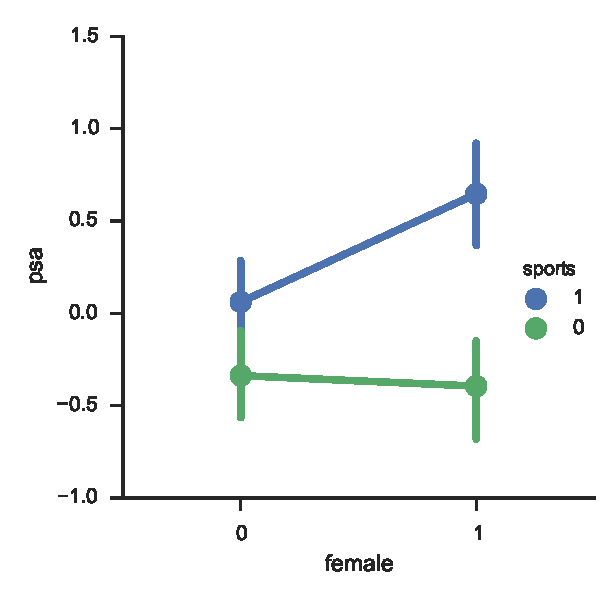
\includegraphics[width=0.5\textwidth]{p3.pdf}
\label{fig:on}
\end{center}
\caption{Effects of biological sex ($female=1, male=0$) and extracurricular activity ($sports=1, other=0$). There is no effect of gender on other extracurriculars, but there is a significant effect of gender on sports extracurriculars. Error bars represent 95\% CI.}
\end{figure}

\clearpage
\problem{}
% http://w3.sista.arizona.edu/~cdawson/ista311/notes/07_relationships_between_RVs.pdf
(10 points) Explain why $r$ must be between -1 and +1. Please, do not use more than 1 or 2 paragraphs. You can append calculations, if you need them.\\

\noindent $r$ is defined as
$$r = \frac{\mbox{cov}_{XY}}{s_X s_Y}.$$
The Cauchy-Schwarz inequality (which I will not prove) states that, for any random variables $A$ and $B$, $\Aver{AB}^2 \leq \Aver{A^2} \Aver{B^2}$. Using $A=X-\mu$ and $B=Y-\nu$, where $\mu=E(X), \nu=E(Y)$, we then have
\begin{align*}
\mbox{cov}_{XY}^2 & = \Aver{(X-\mu)(Y-\nu)}^2 && \text{Definition of covariance.}           \\
                    & \leq \Aver{(X-\mu)^2}\Aver{(Y-\nu)^2}  && \text{Cauch-Schwarz inequality (above).}       \\
                    & \leq s_X^2 s_Y^2  && \text{Definition of variance.}\\
|\mbox{cov}_{XY}|   & \leq \sqrt{s_X^2 s_Y^2}  && \text{Taking positive square roots.}
\end{align*}
This is the same as $-s_X s_Y \leq \mbox{cov}_{XY} \leq s_X s_Y$. The rest is simple algebra
\begin{align*}
-\frac{s_X s_Y}{s_X s_Y} & \leq \frac{\mbox{cov}_{XY}}{s_X s_Y} \leq \frac{s_X s_Y}{s_X s_Y} && \text{Dividing by $s_X s_Y$.}\\
-1 & \leq \frac{\mbox{cov}_{XY}}{s_X s_Y} \leq 1  && \text{Reducing.}\\
-1 & \leq r \leq 1  && \text{Definition of $r$.}
\end{align*}
which was to be proven.

% \clearpage
\problem{}%
% https://stats.stackexchange.com/questions/32464/how-does-the-correlation-coefficient-differ-from-regression-slope
(20 points) Say you run a simple regression with predictor variable $X_1$ and outcome variable $Y$. You fit the following model:
                $$Y = B_0 + B_1 X_1$$
a) What is the interpretation of $B_0$? What is the interpretation of $B_1$?\\
\\
$B_0$ is the intercept---the mean response of Y when $X_1 = 0$. $B_1$ is the slope---the change in mean response in $Y$ when $X_1$ increases by 1 unit. It describes the linear relationship between $X$ and $Y$, which can be positive or negative, and increases with magnitude as the linear relationship becomes stronger.\\
\\
b) When will $B_1$ be equal to the correlation between $Y$ and $X_1$? Why?\\
\\
$B_1$ is equal to the correlation between $Y$ and $X_1$ when the scales of $X$ and $Y$ are the same (for instance, when $X_1$ and $Y$ are standardized).
The slope of our model, $B_1$, is related to the correlation by
\begin{align*}
B_1 &= \mbox{cor}(Y, X_1) \frac{\sigma_Y}{\sigma_{X_1}}
\end{align*}
Therefore the two are equivalent only when $\sigma_{Y} = \sigma_{X_1}$, so the variables must be on the same scale (for instance, again, when $X_1$ and $Y$ are standardized).\\
\\
After running the analysis you remember a covariate that you believe is related to $Y$, but is not substantively of interest.
c) What are the benefits of including the covariate in the model? Include two benefits and explain them in detail.
\begin{enumerate}
\item Increase in power --- adding a covariate can reduce the within-group error variance, increasing the resulting $F$ statistic. When the effects of the covariate on the dependent variable are controlled for, we remove it from the within-group error (denominator of $F$ statistic), making it easier to find a significant effect.
\item Adjust for preexisting differences --- controlling for known extraneous variables, we can gain greater insight into the effect of predictor variables. ANCOVA can adjust for preexisting differences in groups (covariates), making it easier to detect changes in dependent variable.
\end{enumerate}
Finally, you include the covariate within the analysis and fit the following model:
                $$Y = B_0 + B_1 X_1 + B_2 X_2$$
d) What is the interpretation of each of the coefficients in this model?\\
\\
$B_0$ is the intercept---the mean response of Y when $X_1 = X_2 = 0$. $B_1$ is a slope---the change in mean response in $Y$ when $X_1$ increases by 1 unit and $X_2$ is held constant. $B_2$ is also a slope---the change in mean response in $Y$ when $X_2$ increases by 1 unit and $X_1$ is held constant. \\
\\
e) When will $B_1$ be equal to the correlation between $Y$ and $X_1$? When will $B_2$ be equal to the correlation between $Y$ and $X_2$? Why?\\
\\
$B_1$, is related to the correlation by
\begin{align*}
B_1 &= \frac{\mbox{cov}_{Y1} \sigma_2^2 - \mbox{cov}_{Y2} \mbox{cov}_{12}}{\sigma_{2}^2 \sigma_1^2 - \mbox{cov}_{12}^2}  && \text{Definition of regression coefficient.}\\
    &= \frac{\mbox{cov}_{Y1}}{\sigma_{1}^2} && \text{Setting cov$_{12}$ = 0.} \\
\\
r_{Y1}  &= \frac{\mbox{cov}_{Y1}}{\sigma_Y \sigma_1} && \text{Definition of the correlation.}
\end{align*}
Therefore the two are equivalent only when $\sigma_{Y} = \sigma_{1}$, so the variables must be on the same scale (for instance, again, when $X_1$ and $Y$ are standardized). $B_2$, is related to the correlation by
\begin{align*}
B_2 &= \frac{\mbox{cov}_{Y2} \sigma_1^2 - \mbox{cov}_{Y1} \mbox{cov}_{12}}{\sigma_{2}^2 \sigma_1^2 - \mbox{cov}_{12}^2} && \text{Definition of regression coefficient.} \\
    &= \frac{\mbox{cov}_{Y2}}{\sigma_{2}^2} && \text{Setting cov$_{12}$ = 0.} \\
\\
r_{Y2}  &= \frac{\mbox{cov}_{Y2}}{\sigma_Y \sigma_2} && \text{Definition of the correlation.}
\end{align*}
Therefore the two are equivalent only when $\sigma_{Y} = \sigma_{2}$, so the variables must be on the same scale (for instance, again, when $X_2$ and $Y$ are standardized).\\

% \clearpage
\problem{}
(10 points) Suppose you are hired to serve as a statistical consultant. In each of the following cases, what advice (if any) would you give to your client concerning the procedures and/or conclusions he or she has drawn, or about the kind of statistical techniques most suitable? Be sure to briefly explain the reasoning underlying your advice.\\
\\
(a) A researcher studies the effects of education (HS or less, Some College, 4 Year College Degree, Graduate/Professional Degree) on income by randomly calling 5,000 participants in the United States. At a presentation of his results several colleagues suggest that effects of education on income may not be robust when considering other predictors such as work experience, time with their current employer, age, personal investments. What sort of analysis did the researcher conduct, and how can the researcher address these criticisms of his research?\\
\\
As the researcher was studying a single factor's effect on a single outcome variable, they most likely performed a single factor ANOVA. This single factor ANOVA investigated the effect of a categorical variable, education level, on a continuous outcome variable, income. His colleagues are asking why he did not perform a factorial ANOVA to test the effects of additional potential predictors. The researcher should agree with these criticisms, as his results will not be robust to other predictors. Hopefully this researcher has looked in the literature and found that these predictors do not have much influence (in which case he could potentially get away with not looking). It's also possible that the researcher could claim that, due to budget, time, or other constraints, it was impossible to take additional data. If it was possible to ask his participants additional questions, the researcher should have taken advantage of a factorial design to reduce their unexplained variance, and draw additional conclusions (main effects, interactions, etc).\\
\\
(b) A researcher is interested in predicting the mental health of college students based on their reported level of stress. What kind of sample should she collect and what statistical technique should she use to achieve this goal?\\
\\
The researcher should randomly sample from all college students. Since this is probably impossible, the researcher may be better off advertising their study to a select few local colleges. The researcher would then need to record data on each subject's mental health, reported stress level, and college. Additional questions could (and should) be asked, such as the subject's age and gender, since it's simple to gather this data simultaneously, and may have important interaction effects on the results. Taking this approach, the researcher should use an ANCOVA design to determine the effects of stress and other measured covariates on mental health.\\
\\
(c) A researcher collected data from undergraduate and graduate students at universities across the country in a study of the relation between age (Range of 18-46 years with a Mean = 23.5) and openness. There was a significant, negative relation between age and openness $(r(2,998) = -0.13, p < .05)$. The researcher cited this finding as evidence for why elderly individuals (age 60 years and upward) have difficulty learning about novel technology and ideological shifts; they're openness has declined substantially over their lives. Is this a reasonable conclusion? Why or why not?\\
\\
This is not a reasonable conclusion. The researcher is taking findings from one population (students between ages 18-46) and extending them onto another population (the elderly, ages $\geq60$). The elderly were not sampled in the study, so it is unwise to extend results to their age group. A significant, negative relation between age and openness may exist among university students, but this linear relationship may not continue outside their age group. Furthermore, no correlation between learning novel technology (or ideological shifts) and openness was found in the university students. Simply put, the researcher is reaching too far with their conclusions---there is no evidence that the relation between age and openness continues past the measured age group, and there is no measured correlation between learning novel technology and openness.\\
\\
(d) A researcher studied a group of 100 students by having them complete a survey once a quarter, every quarter, for two years via an online survey form. The survey consisted of several items meant to measure anxiety, self-competence, and academic performance. What methods of analysis would be applicable to this type of data? How do you justify your recommendations?\\
\\
This type of study could be analyzed with repeated measures ANOVA, but it is probably better to use mixed effects models. Since we're doing research with students over a long period of time, it is likely that many of them will fail to complete the entire experiment. A repeated measures ANOVA could be used here, but the researcher would have to drop all the subjects that did not complete the entire experiment, which could lead to unintentional biases in the results (perhaps the students that dropped out had poor academic performance). A mixed effects model can use subjects that drop out, or simply miss a session. Mixed effects models also don't require an assumption of sphericity, which can often be violated in longitudinal studies.\\
\\
(e) A researcher received a small grant to conduct a study and is debating on how to spend the money. She is thinking that she can give a test to 300 individuals on one occasion, give a test to one individual on 300 occasions, give a test to 30 individuals on 10 occasions, give a test to 10 individuals on 30 occasions, or any combination of the above. Which of these data collection methods should she use?\\
\\
The solution, of course, depends on what the researcher is researching (and how small the grant is). Each of these methods is perfectly valid, but the results that can be drawn from the different data collections methods will vary. Most of these methods (with the exception of the first), involve taking multiple measurements from individual(s). These methods will allow the researcher to conduct repeated measures tests on their data. If the researcher is not interested in changes with respect to time, they should probably choose the first method. If the researcher has enough money to think that ``any combination of the above'' methods is a valid choice, then they should choose \textit{all} of the methods. That being said, no good answer can be given to this question without knowing more about what is being researched.

% \clearpage
\problem{Extra Credit}

(10 points) Explain what it means to say that a correlation is a covariance expressed in z-scores? Derive numerically the formula for a correlation based on the formula from a covariance (and describe the steps in your own words).\\
\\
You must know the variance of a variable to determine the meaning of a covariance value. To remove this requirement, the covariance can be scaled by the standard deviations of the covarying variables to convert the covariance value to a correlation value. It's easier to draw conclusions from correlation scores as they are bound by $\pm 1$ (see previous problem).

\begin{align*}
\mbox{cor}(X, Y) &= \mbox{cov}\left( Z_X, Z_Y \right) && \text{Given the correlation of X, Y is equal to the} \\
& && \text{covariance of $Z_X$ and $Z_Y$.} \\
\mbox{cor}(X, Y) &= \mbox{cov} \left(\frac{X - \Aver{X}}{\sigma_X}, \frac{Y - \Aver{Y}}{\sigma_Y} \right) && \text{Expand $Z_X$ and $Z_Y$ by the definition of z-scores.}\\
\mbox{cor}(X, Y) &= \frac{\Aver{\left(X - \Aver{X} \right) \left(Y - \Aver{Y} \right) }}{\sigma_X \sigma_Y} && \text{Definition of covariance.} \\
\mbox{cor}(X, Y) &= \Aver{\frac{X - \Aver{X}}{\sigma_X } \frac{Y - \Aver{Y} }{\sigma_Y}} && \text{Regrouping.} \\
\mbox{cor}(X, Y) &= \frac{\mbox{cov}(X, Y)}{\sigma_X \sigma_Y} && \text{Which is the definition of the correlation.} \\
\end{align*}


% \begin{align*}
% \mbox{cor}(X, Y) &= \frac{\mbox{cov}(X, Y)}{\sigma_X \sigma_Y} && \text{Definition of correlation.}\\
%                  &= \frac{\Aver{\left(X - \Aver{X} \right) \left(Y - \Aver{Y} \right) }}{\sigma_X \sigma_Y} && \text{Definition of covariance.}\\
%                  &= \Aver{\frac{X - \Aver{X}}{\sigma_X} \frac{Y - \Aver{Y}}{\sigma_Y}}  && \text{Algebraic rearranging.}\\
%                  % &= \Aver{\frac{X}{\sigma_X} \frac{Y}{\sigma_Y}}
%                  &= \Aver{Z_X Z_Y}  && \text{Definition of z-score.}
% \end{align*}



\end{document}
